% PLANO DE TRABALHO------------------------------------------------------------------

\chapter{PLANO DE TRABALHO}
\label{chap:metodologia}
Alguns conceitos de processamento de imagens foram apresentados até o momento, bem como algumas técnicas de inteligência artificial que podem ser utilizadas na etapa de reconhecimento e interpretação. 

A proposta deste trabalho visa a utilização de metodologias de aprendizado de máquina, sendo aplicado conceitos de aprendizado profundo supervisionado, de maneira a reduzir tempo de processamento e obter um aumento nos resultados de acurácia a partir de resultados apresentados por \citeonline{Paglione2016}. Em seu trabalho, \citeonline{Paglione2016} apresenta uma proposta de melhoria em resultados de acurácia e tempo para o teste de tetrazólio utilizando técnicas de PDI, por meio de diferentes métodos de segmentação de imagem.

\section{METODOLOGIA PROPOSTA}
\label{sec:titSecMetProposta}

Para o presente trabalho será utilizado uma base de imagens de sementes de soja provenientes do trabalho desenvolvido por \citeonline{Santanna2014}. Porém serão aplicadas técnicas de processamento de imagem propostos por \citeonline{Paglione2016}, o \textit{pipele} de execução é apresentado na \autoref{fig:figura-pipelinePreProcessamento}, das quais mostraram resultados otimizados em relação ao trabalho apresentado por \citeonline{Santanna2014}.

\begin{figure}[!htb]
    \centering
    \caption{Pipeline do pré-processamento}
    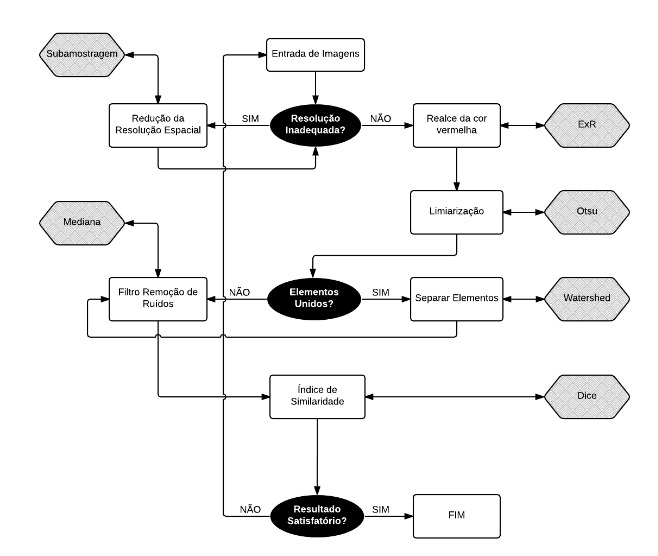
\includegraphics[width=1\textwidth]{./dados/figuras/pipeline-paglione.jpeg}
    \fonte{}
    \label{fig:figura-pipelinePreProcessamento}
\end{figure}

A aquisição das imagens é dada a partir da base de dados composta por lâminas de sementes de soja. A primeiro momento é verificado a resolução das imagens de entrada, caso seja inapropriadamente alta, está será reduzida utilizando o método \textit{downsampling}.

\subsection{PRÉ-PROCESSAMENTO}
\label{sec:titSubSecPreProcessamento}

Como descrito na \autoref{sec:titSecAnalSementes}, a solução do teste de tetrazólio proporciona uma cor avermelhada as sementes de soja submetidas, e está cor caracteriza o resultado do teste. Em função disso, será realçada a cor vermelha, para melhor proveito do conceito de índice de vegetação ExR, excesso de vermelho (do inglês, \textit{Excess Red}), a fim de uma melhor análise dos resultados. E então realizada uma limiarização de Otsu, com o objetivo de segmentar as imagens de semente de soja do fundo, proporcionando uma cor branca as sementes e ao fundo da imagem, a cor preta. Caso a imagem resultante ainda conter elementos conectados entre si é aplicado o algoritmo de segmentação de \textit{watershed}. E por fim, aplicado o filtro de mediana para remoção de possíveis ruídos.

Para a etapa de representação e descrição será utilizado um \textit{script} desenvolvido na linguagem python que agrupará as imagens em \textit{clusters} semelhantes utilizando-se técnicas de aprendizado de máquina, além do auxílio da API Keras. A Keras é uma biblioteca de \textit{Deep Learning} de alto nível desenvolvida em python, capaz de executar em uma camada acima da TensorFlow - biblioteca de código aberto para aprendizado de máquina, desenvolvida pela Google. A biblioteca dispõe de modelos de aprendizado profundo, pré-treinados por imagens da ImageNet, que serão utilizados para extração de um vetor com as características das imagens.

\subsection{FLORESTA DE CAMINHOS ÓTIMOS}
\label{sec:titSubSecOPF}

A etapa de reconhecimento e interpretação, como citado anteriormente na \autoref{sec:titSecVisaoComputacional}, envolve a realização de aprendizado e representar os padrões aprendidos. Para isso, este trabalho tem como objetivo propor e desenvolver uma nova técnica de aprendizado supervisionado por meio de variáveis latentes. Para tanto, a mesma será baseada no conceito de Floresta de Caminhos Ótimos (OPF, do inglês \textit{Optimum Path Forest}), o qual apresenta resultados eficazes e eficientes quando comparado com outros algoritmos de aprendizado supervisionado da literatura (PAPA, 2008).

As florestas de caminhos ótimos embasam-se no conceito de otimização de caminhos por meio do algoritmo de Dijkstra
contendo múltiplas fontes e sumidouros. Dessa forma, o classificador supervisionado OPF consiste em um arcabouço para instanciação de classificadores baseados nas florestas de caminhos ótimos. Os métodos de aprendizado suportados por tal arcabouço são o supervisionado e o não-supervisionado, neste trabalho foi utilizado o método de aprendizado supervisionado com uma abordagem de grafo completo.

Vale ressaltar que, a maioria dos classificadores na literatura geralmente apresentam boa eficácia a partir de um grande conjunto de dados de treinamento, já a OPF mostrou-se eficaz, na maioria das vezes, bem como eficiente em treinamentos e testes independentemente do tamanho do conjunto de dados. 

Após as \textit{deep features} serem extraídas das imagens as mesmas foram organizadas em vetores de características. A OPF modela cada vetor como sendo um nó de um grafo completo, ou seja, todos os nós devem estar conectados. O algoritmo de treinamento encarrega-se de escolher os protótipos de cada classe (raízes de cada árvore de caminho ótimo). Esses, por sua vez, tentarão conquistar os outros nós não-protótipos. Um custo é atribuído a cada nó não-protótipo e a aresta que apresentar o menor custo entre o nó protótipo, conquista a amostra atribuindo a essa o rótulo da classe.

Os passos realizados pela abordagem proposta são explicitados na Figura 3. No passo 1, todas as amostras são conectadas e definidos os protótipos de cada classe (ilustrados pela borda pontilhada), em seguida é calculado o peso de cada aresta. Para cada nó é definido também uma função de custo, após isso os nós protótipos irão tentar conquistar as demais amostras, o protótipo que oferecer o menor custo à outra amostra, conquista a amostra. No passo 2, é ilustrado o processo após o treinamento, onde o
protótipo A conquistou a amostra B e o protótipo C conquistou a amostra D. No passo 3, é ilustrado a fase de teste, onde uma nova amostra teste será conectada aos demais nós da rede e essa será conquistada pela amostra que lhe oferecer o menor custo, na
Figura 3 temos que a amostra X será conquistada pelo nó A.

\begin{figure}[!htb]
    \centering
    \caption{Fase de teste da OPF}
    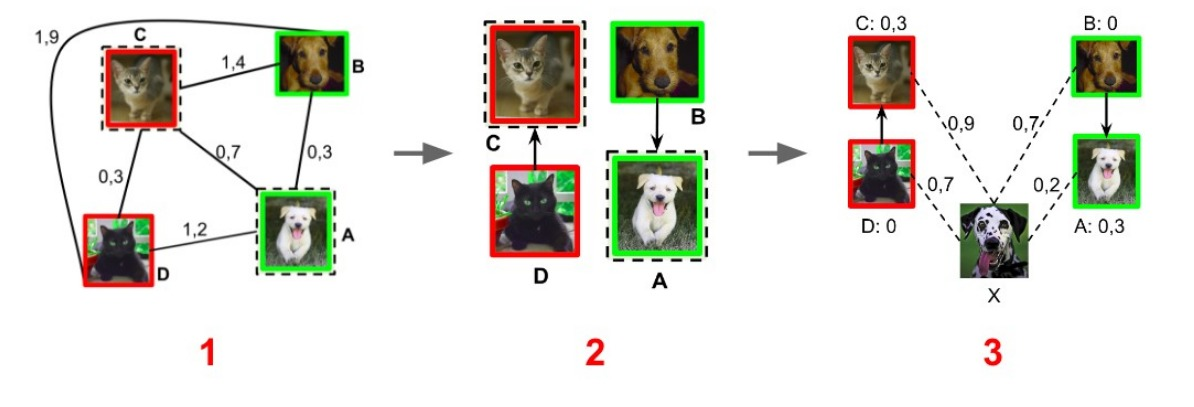
\includegraphics[width=1\textwidth]{./dados/figuras/opf-funcionamento.jpeg}
    \fonte{Autoria própria}
    \label{fig:figura-FaseTesteOPF}
\end{figure}

\subsection{ANÁLISE DE VARIÁVEIS LATENTES}
\label{sec:titSubSecVarLatentes}

Uma variável latente auxilia no fato de que não é necessário comparar inúmeras correlações para encontrar padrões, empregando apenas algumas técnicas estatísticas é possível inferir padrões (ANDRADE et al., 2014).

Para realizar a identificação de variáveis latentes no contexto de análise de imagens foi então utilizado o conceito de floresta de caminhos ótimos, o qual calcula a distância entre cada nó da etapa de treinamento e teste. Dessa forma, a partir de tais informações pôde-se utilizar tais distâncias para propor e calcular uma formulação para pertinência de cada sub-imagem a cada uma das classes abordadas em um dado contexto. A partir de tal formulação é possível obter relevância de uma dada amostra (i.e. sub-imagem) pertencer ou não às classes abordadas no problema. Tal informação é obtida facilmente por meio do menor valor correspondente na lista de distâncias, representada por h+, e menor valor com classe diferente da sub-imagem na lista de distâncias, denotada por h-. A pontuação é dada a partir da \autoref{eq:equacao-score}.

\begin{equation}
    score = |\, ({h}^{+}) \, - \, ({h}^{-}) \, |
    \label{eq:equacao-score}
\end{equation}

As pontuações de todas as sub imagens são armazenadas e comparadas, com o intuito de identificar quais fragmentos da imagem original obtiveram maior e menor pontuação. Sendo possível obter as variáveis latentes, dada a maior e menor pontuações.

\section{RESULTADOS ESPERADOS}
\label{sec:titSecResultEsperados}

Espera-se desenvolver uma técnica capaz de realizar o aprendizado
profundo de máquina, solucionando o erro de mapeamento dos classificadores atuais, empregando métodos e os respectivos passos que foram descritos na \autoref{sec:titSecMetProposta}.

Analisar qual o método mais eficiente da biblioteca Keras, para extração de características, que trará os melhores resultados. E analisar a eficiência da biblioteca da OPF e quais parâmetros permitem desenvolver um classificador que retorne os resultados esperado para o teste de tetrazólio.

Entender, por meio das variáveis latentes, quais fatores desencadeiam uma classificação equivocada, para a base de imagens utilizada.

Obter bons resultados que permitam que o classificador atenda as expectativas humanas no teste de tetrazólio.

